%----------------------------------------------------------------------------------------
%	SECTION 1
%----------------------------------------------------------------------------------------


% Lorem ipsum dolor sit amet, consectetur adipiscing elit. Aliquam ultricies lacinia euismod. Nam tempus risus in dolor rhoncus in interdum enim tincidunt. Donec vel nunc neque. In condimentum ullamcorper quam non consequat. Fusce sagittis tempor feugiat. Fusce magna erat, molestie eu convallis ut, tempus sed arcu. Quisque molestie, ante a tincidunt ullamcorper, sapien enim dignissim lacus, in semper nibh erat lobortis purus. Integer dapibus ligula ac risus convallis pellentesque.

% \begin{figure}
% \centering
% \begin{subfigure}{.5\textwidth}
%   \centering
%   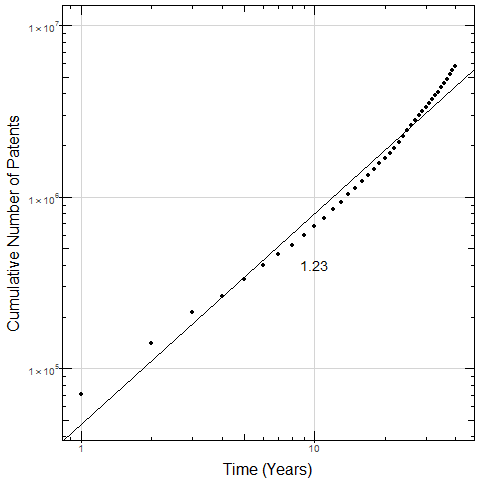
\includegraphics[width=0.7\linewidth]{Figures/CumulativePatents1}
%  \caption[CumPatents1]{\small Generalised linear model $y = x^\alpha $, fitted to all the data-points}
% \label{fig:CumPatents1}
% \end{subfigure}%
% \begin{subfigure}{.5\textwidth}
%   \centering
%   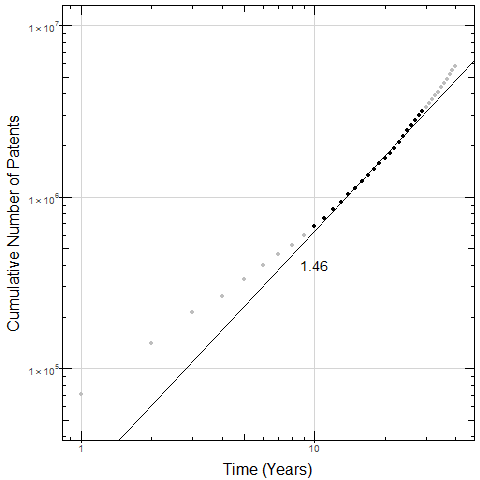
\includegraphics[width=0.7\linewidth]{Figures/CumulativePatents2}
%   \caption[CumPatents1]{\small Generalised linear model $y = x^\alpha $, fitted only to the years 1986 to 2005}
% \label{fig:CumPatents2}
% \end{subfigure}
% \caption[Power-law fit for cumulative number of patents granted each year]{The cumulative number of patents granted from 1976 to 2015, plotted on a log-log scales}
% \label{fig:CumPatents}
% \end{figure}

% %-----------------------------------
% %	SUBSECTION 1
% %-----------------------------------

% Nunc posuere quam at lectus tristique eu ultrices augue venenatis. Vestibulum ante ipsum primis in faucibus orci luctus et ultrices posuere cubilia Curae; Aliquam erat volutpat. Vivamus sodales tortor eget quam adipiscing in vulputate ante ullamcorper. Sed eros ante, lacinia et sollicitudin et, aliquam sit amet augue. In hac habitasse platea dictumst.

% \begin{figure}
% \centering
% \begin{subfigure}{.3\linewidth}
%   \centering
%   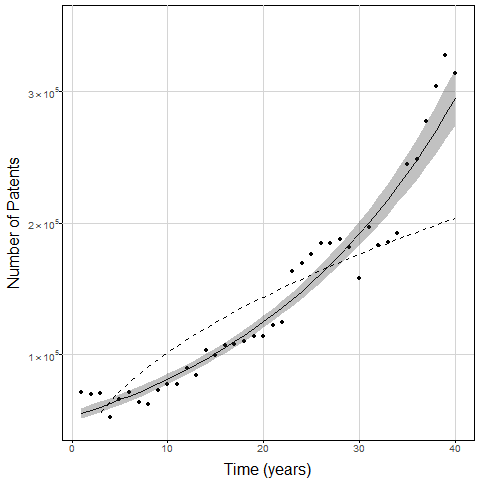
\includegraphics[width=0.9\linewidth]{Figures/patentCountFit}
%  \caption[CumPatents1]{\footnotesize Patents granted per year}
% \label{fig:patentCountFit}
% \end{subfigure}%
% \begin{subfigure}{.3\linewidth}
%   \centering
%   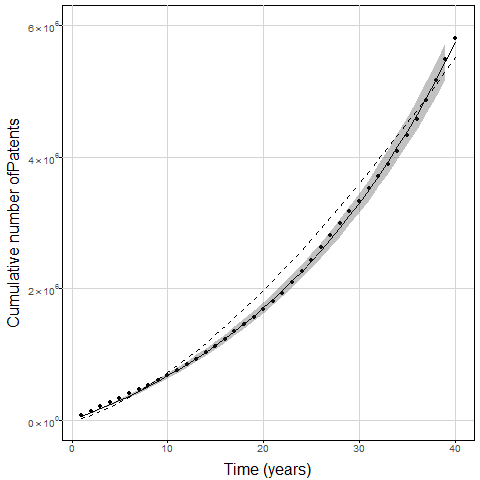
\includegraphics[width=0.9\linewidth]{Figures/patentCountFit_cum}
%   \caption[CumPatents1]{\footnotesize Cumulative number of patents granted}
% \label{fig:patentCountFit_cum}
% \end{subfigure}
% \begin{subfigure}{.3\linewidth}
%   \centering
%   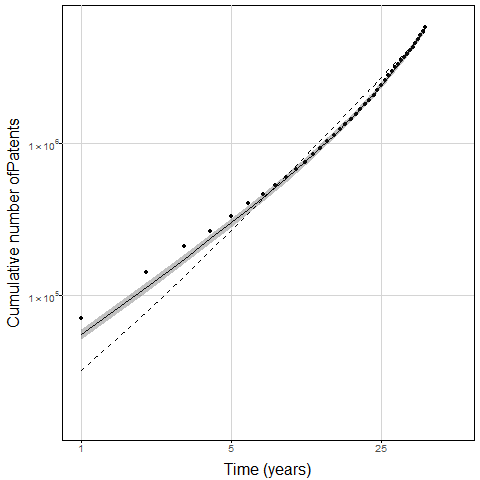
\includegraphics[width=0.9\linewidth]{Figures/patentCountFit_cum_loglog}
%   \caption[CumPatents1]{\footnotesize Cumulative patents granted on a log-log scale}
% \label{fig:patentCountFit_cum_loglog}
% \end{subfigure}
% \caption[Exponential fit for number of patents granted each year]{Power law and exponential fits for cumulative number of patents published each year}
% \label{fig:cumulativePatentFits}
% \end{figure}

%-----------------------------------
%	SUBSECTION 2
%-----------------------------------

% Morbi rutrum odio eget arcu adipiscing sodales. Aenean et purus a est pulvinar pellentesque. Cras in elit neque, quis varius elit. Phasellus fringilla, nibh eu tempus venenatis, dolor elit posuere quam, quis adipiscing urna leo nec orci. Sed nec nulla auctor odio aliquet consequat. Ut nec nulla in ante ullamcorper aliquam at sed dolor. Phasellus fermentum magna in augue gravida cursus. Cras sed pretium lorem. Pellentesque eget ornare odio. Proin accumsan, massa viverra cursus pharetra, ipsum nisi lobortis velit, a malesuada dolor lorem eu neque.


% \begin{figure}
% \centering
% \begin{subfigure}{.5\textwidth}
%   \centering
%   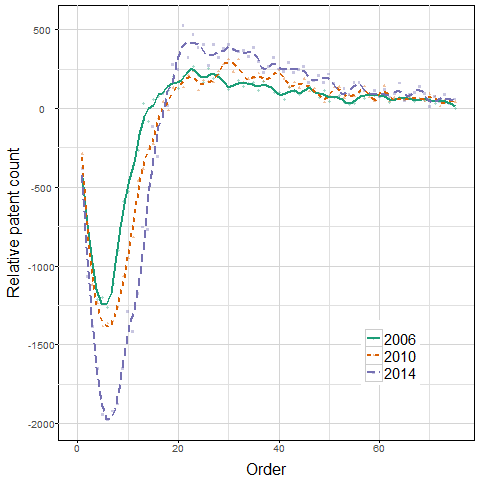
\includegraphics[width=0.7\linewidth]{Figures/parsingErrorsPerOrder}
%  \caption[CumPatents1]{\small Generalised linear model $y = x^\alpha $, fitted to all the data-points}
% \label{fig:parsingErrorsPerOrder}
% \end{subfigure}%
% \begin{subfigure}{.5\textwidth}
%   \centering
%   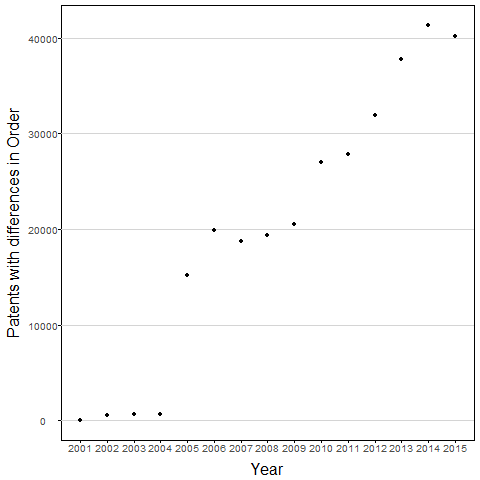
\includegraphics[width=0.7\linewidth]{Figures/parsingErrorsPerYear}
%   \caption[CumPatents1]{\small Generalised linear model $y = x^\alpha $, fitted only to the years 1986 to 2005}
% \label{fig:parsingErrorsPerYear}
% \end{subfigure}
% \caption[Differences in different parsing methods]{Number of patents with different values for order computed by (1) when parsing original data, (2) using a mapReduce on citations table.}
% \end{figure}

%----------------------------------------------------------------------------------------
%	SECTION 2
%----------------------------------------------------------------------------------------

% \section{Main Section 2}

% Sed ullamcorper quam eu nisl interdum at interdum enim egestas. Aliquam placerat justo sed lectus lobortis ut porta nisl porttitor. Vestibulum mi dolor, lacinia molestie gravida at, tempus vitae ligula. Donec eget quam sapien, in viverra eros. Donec pellentesque justo a massa fringilla non vestibulum metus vestibulum. Vestibulum in orci quis felis tempor lacinia. Vivamus ornare ultrices facilisis. Ut hendrerit volutpat vulputate. Morbi condimentum venenatis augue, id porta ipsum vulputate in. Curabitur luctus tempus justo. Vestibulum risus lectus, adipiscing nec condimentum quis, condimentum nec nisl. Aliquam dictum sagittis velit sed iaculis. Morbi tristique augue sit amet nulla pulvinar id facilisis ligula mollis. Nam elit libero, tincidunt ut aliquam at, molestie in quam. Aenean rhoncus vehicula hendrerit.

% \begin{figure}
% \centering
%  \centering
%  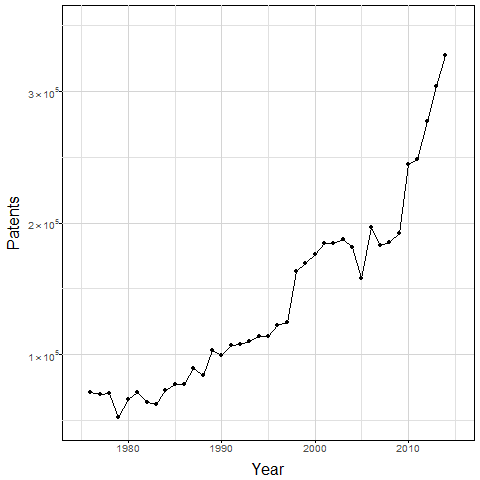
\includegraphics[width=0.7\linewidth]{Figures/PatentCountVsYear}
% \caption[Number of patents granted each year]{Number of patents granted each year from 1976 to 2015}
% \label{fig:PatentCountVsYear}
% \end{figure}

% \begin{figure}
% \centering
%   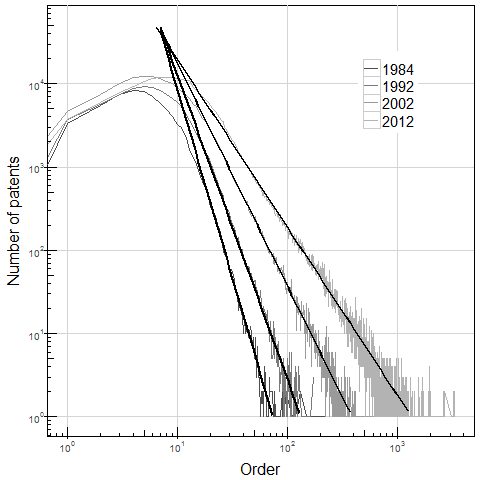
\includegraphics[width=0.7\linewidth]{Figures/OrderDistribution}
%   \caption[Degree Distribution]{Degree distribution (number of citations for each patent) on a log-log scale shown for years 1984,1992,2002,2012. Fit with generalized linear model of the form $y ~ x^\alpha$ yielding exponents of -...,-...,-... and -... respectively}
% \label{fig:OrderDistribution}
% \end{figure}

%----------------------------------------------------------------------------------------
%	SECTION 3
%----------------------------------------------------------------------------------------

% \section{Main Section 3}

% Sed ullamcorper quam eu nisl interdum at interdum enim egestas. Aliquam placerat justo sed lectus lobortis ut porta nisl porttitor. Vestibulum mi dolor, lacinia molestie gravida at, tempus vitae ligula. Donec eget quam sapien, in viverra eros. Donec pellentesque justo a massa fringilla non vestibulum metus vestibulum. Vestibulum in orci quis felis tempor lacinia. Vivamus ornare ultrices facilisis. Ut hendrerit volutpat vulputate. Morbi condimentum venenatis augue, id porta ipsum vulputate in. Curabitur luctus tempus justo. Vestibulum risus lectus, adipiscing nec condimentum quis, condimentum nec nisl. Aliquam dictum sagittis velit sed iaculis. Morbi tristique augue sit amet nulla pulvinar id facilisis ligula mollis. Nam elit libero, tincidunt ut aliquam at, molestie in quam. Aenean rhoncus vehicula hendrerit.

% \begin{figure}
% \centering
% \begin{subfigure}{.5\textwidth}
%   \centering
%   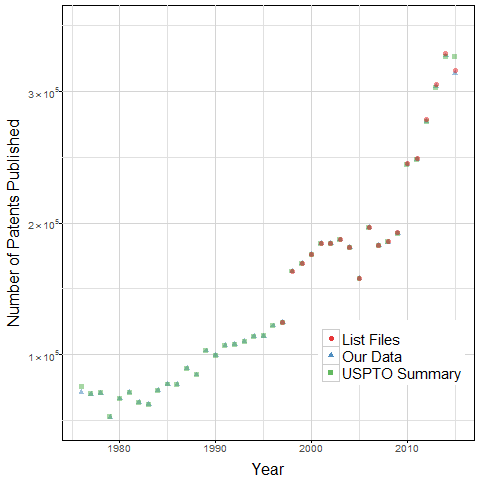
\includegraphics[width=0.7\linewidth]{Figures/patentsCompared}
%  \caption{Number of Patents parsed each year from each source}
% \label{fig:patentsCompared}
% \end{subfigure}%
% \begin{subfigure}{.5\textwidth}
%   \centering
%   
\includegraphics[width=0.7\linewidth]{Figures/patentsDiff}
%   \caption{\footnotesize Difference between number of Patents parsed from different sources and parsed data}
% \label{fig:patentsDiff}
% \end{subfigure}
% \caption[Difference between number of patents parsed from different sources]{\footnotesize The number of Patents granted each year according to 3 sources: Parsed data; a USPTO report and the .lst files.}
% \label{fig:patentCountsTest}
% \end{figure}